\documentclass[11pt,a4paper]{article}

\usepackage[utf8]{inputenc}
\usepackage[T1]{fontenc}
% Latin Modern incluye fuentes vectoriales T1 y evita depender de que TinyTeX
% genere fuentes bitmap durante la compilación en equipos sin permisos globales.
\usepackage{lmodern}
\usepackage[provide=*,spanish]{babel}
\usepackage{amsmath,amssymb}
\usepackage{booktabs}
\usepackage{tabularx}
\usepackage{array}
\usepackage{graphicx}
\usepackage{geometry}
\usepackage{xcolor}
\usepackage{float}
\usepackage{hyperref}
\usepackage{url}

% El documento se compila desde zombie_poisson_streamlit/report. Las figuras
% y tablas se regeneran con generate_report_assets.py para que el informe use
% exactamente el mismo motor estadístico que la aplicación.
\graphicspath{{../assets/}}
% Archivo generado automáticamente; no editar a mano.
\newcommand{\ResultsDate}{2026-09-04}
\newcommand{\PoissonSurvival}{35.2}
\newcommand{\PolarSurvival}{77.8}
\newcommand{\PoissonCILow}{30.7}
\newcommand{\PoissonCIHigh}{40.1}
\newcommand{\PolarCILow}{73.4}
\newcommand{\PolarCIHigh}{81.6}
\newcommand{\PoissonMeanTime}{64.694}
\newcommand{\PolarMeanTime}{83.666}
\newcommand{\PoissonPeak}{14.220}
\newcommand{\PolarPeak}{11.225}
\newcommand{\SurvivalDifference}{-42.5}
\newcommand{\SurvivalDiffLow}{-48.8}
\newcommand{\SurvivalDiffHigh}{-35.8}
\newcommand{\McNemarP}{1.697\times 10^{-28}}
\newcommand{\PeakDifference}{2.995}
\newcommand{\PeakP}{7.007\times 10^{-39}}
\newcommand{\TestCount}{18}
\newcommand{\SmallestNominalP}{0.1716}
\newcommand{\ExponentialKSP}{0.1863}
\newcommand{\NormalKSP}{0.9236}
\newcommand{\AcceptanceRate}{0.7765}
\newcommand{\AcceptanceP}{0.1716}
\newcommand{\LognormalMeanP}{0.7158}
\newcommand{\CountDispersionP}{0.3464}
\newcommand{\CountChiP}{0.7887}
\newcommand{\UniformKSP}{0.3006}
\newcommand{\UniformSerialP}{0.4918}
\newcommand{\LcgKSP}{0.8062}
\newcommand{\LcgSerialP}{0.6986}
\newcommand{\ControlUniformityP}{0.9999}
\newcommand{\ControlKSP}{1.0000}
\newcommand{\ControlRunsP}{<10^{-16}}
\newcommand{\ControlLjungP}{<10^{-16}}
\newcommand{\ControlSerialP}{<10^{-16}}
\newcommand{\PoissonMicros}{0.040}
\newcommand{\PolarMicros}{0.147}
\newcommand{\PolarNormalKSP}{0.1337}
\newcommand{\BoxMullerKSP}{0.3288}
\newcommand{\PolarNormalMicros}{0.105}
\newcommand{\BoxMullerMicros}{0.051}
\newcommand{\PolarRejectedPercent}{21.8}
\newcommand{\NormalMethodWinner}{Box-Muller}
\newcommand{\PolarMethodScore}{3.908}
\newcommand{\BoxMullerMethodScore}{4.800}
\newcommand{\BothSurvive}{99}
\newcommand{\OnlyPoisson}{42}
\newcommand{\OnlyPolar}{212}
\newcommand{\BothFail}{47}


\geometry{margin=2.35cm,headheight=16pt}
\definecolor{outbreakgreen}{HTML}{567D35}
\definecolor{outbreaklime}{HTML}{B8F36B}
\definecolor{outbreakdark}{HTML}{0B100D}
\definecolor{outbreakpanel}{HTML}{EEF3EE}
\definecolor{outbreakblue}{HTML}{3D7F99}
\definecolor{outbreakink}{HTML}{202923}
\definecolor{outbreakmuted}{HTML}{617067}

\hypersetup{
  colorlinks=true,
  linkcolor=outbreakgreen,
  citecolor=outbreakblue,
  urlcolor=outbreakblue,
  pdftitle={Outbreak: Stochastic Survival Lab},
  pdfauthor={Grupo 1, Sección 30}
}
\setlength{\parskip}{0.55em}
\setlength{\parindent}{0pt}
\renewcommand{\arraystretch}{1.18}

\pagestyle{plain}

\newcommand{\callout}[2]{%
  \begin{center}
  \fcolorbox{outbreakgreen}{outbreakpanel}{%
    \begin{minipage}{0.91\textwidth}
      \textbf{\textcolor{outbreakgreen}{#1}}\quad #2
    \end{minipage}}
  \end{center}}

\begin{document}

% Portada construida con la lista oficial de integrantes del equipo.
\hypersetup{pageanchor=false}
\begin{titlepage}
\pagecolor{outbreakdark}
\color{white}
\centering
\vspace*{0.7cm}
{\small\bfseries\textcolor{outbreaklime}{UNIVERSIDAD DEL VALLE DE GUATEMALA}\par}
\vspace{0.25cm}
{\small CC2017 -- Modelación y Simulación · Sección 30\par}
\vspace{1cm}
{\Huge\bfseries OUTBREAK\par}
\vspace{0.18cm}
{\LARGE\bfseries\textcolor{outbreaklime}{STOCHASTIC SURVIVAL LAB}\par}
\vspace{0.45cm}
{\large Simulación, validación y comparación de métodos de generación\par}
\vspace{0.7cm}
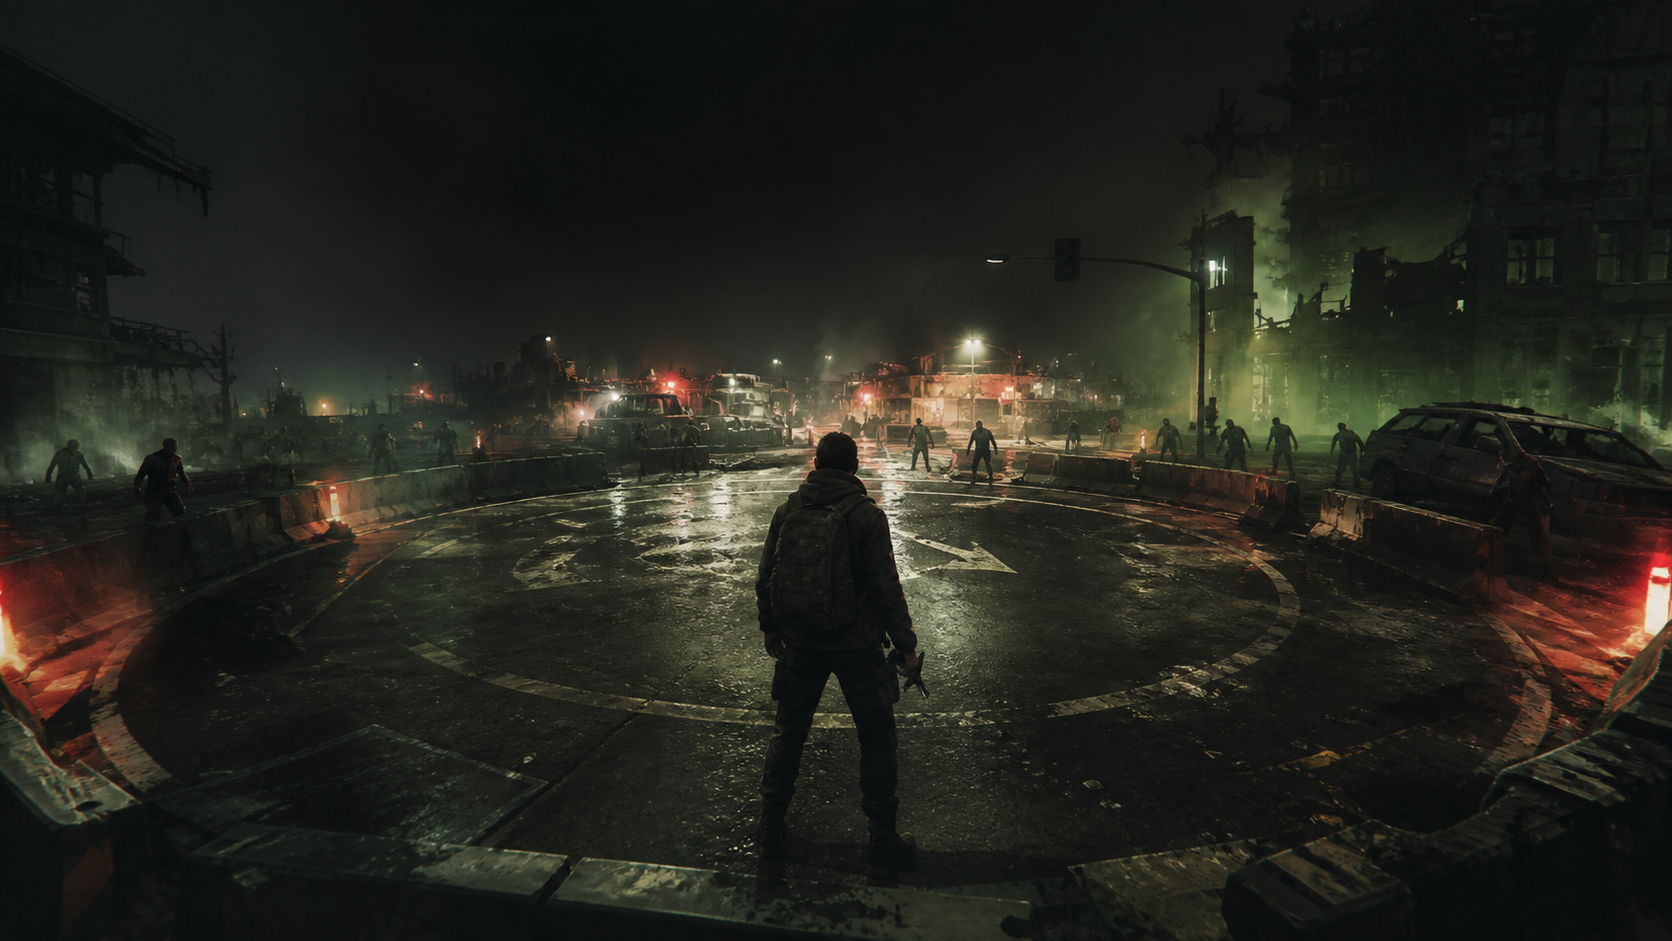
\includegraphics[width=0.88\textwidth]{outbreak-command-center.png}
\vfill
{\normalsize
Pablo Daniel Barillas Moreno · Jorge Palacios\par
Adrián Ricardo González Muralles\par
Andrés Rafael Chivalán · Javier Andrés Chen\par}
\vspace{0.55cm}
{\small Proyecto de curso · Agosto de 2026\par}
\end{titlepage}
\hypersetup{pageanchor=true}
\nopagecolor
\color{outbreakink}

\begin{abstract}
Este trabajo modela un subsistema real de un videojuego de supervivencia: la
aparición, desplazamiento y presión concurrente de enemigos durante una misión.
El modelo principal es un proceso de Poisson homogéneo cuyos interarribos
exponenciales se generan por transformada inversa. Como contraste se implementa
un proceso de renovación con interarribos lognormales; las normales auxiliares
se obtienen mediante Marsaglia Polar. Ambos modelos comparten tiempo medio entre
llegadas, pero difieren en variabilidad y memoria.

Para satisfacer una comparación algorítmica controlada, Marsaglia Polar también
se enfrenta a Box--Muller generando la misma $N(0,1)$. Esta separación evita
atribuir a un algoritmo las diferencias que en realidad proceden de dos
distribuciones de interarribo distintas.

La versión auditada valida la cadena completa: primero la fuente uniforme que
alimenta a ambos métodos, después las transformaciones y por último el conteo del
calendario, con \TestCount{} contrastes sin duplicar el mismo estadístico y corrección
por multiplicidad; comparación pareada con McNemar, Wilcoxon y bootstrap;
intervalos de Wilson; benchmark de generación; corrección del límite temporal;
figuras reproducibles y una escena tridimensional. En el escenario base,
Poisson alcanzó \PoissonSurvival\,\% de supervivencia y Polar-lognormal
\PolarSurvival\,\%. El efecto Poisson menos Polar fue
\SurvivalDifference\ puntos porcentuales, con IC bootstrap
[\SurvivalDiffLow, \SurvivalDiffHigh] y $p=\McNemarP$. Los datos completos
se distribuyen como CSV y pueden regenerarse desde el código.
\end{abstract}

\tableofcontents
\newpage

\section{Descripción del sistema}

\subsection{Sistema real modelado}

La narrativa utiliza un apocalipsis zombi, pero el objeto técnico es el
\textbf{subsistema de aparición y balance de enemigos de un videojuego}. Este
tipo de sistema real de software decide cuándo aparece una entidad, qué
atributos recibe y cómo la presión acumulada afecta la dificultad. Reemplazar
apariciones periódicas por variables aleatorias evita patrones memorizables y
permite cuantificar el balance por simulación.

El protagonista permanece en el centro de una arena. Los infectados nacen cerca
del perímetro, avanzan radialmente y agregan su DPS al daño entrante cuando
alcanzan el radio de contacto. El protagonista ataca un objetivo a la vez. La
misión termina al alcanzar $T$ con HP positivo o al agotar la vida.

\callout{Pregunta de investigación}{¿Cómo cambian congestión, supervivencia y
costo computacional cuando se conserva la tasa media, pero se modifica el
método y la distribución de los interarribos?}

\subsection{Alcance}

El motor procesa un calendario y actualiza combate con paso fijo. No pretende
ser un motor formal de eventos discretos, formalismo que las instrucciones del
curso declaran innecesario en esta etapa. Ruinas, vehículos y barricadas
aportan contexto visual, pero no alteran trayectorias. Las salidas son
supervivencia, tiempo resistido, llegadas, eliminaciones y concurrencia máxima.

\section{Objetivos}

\subsection{Objetivo general}

Diseñar, implementar y analizar una simulación reproducible del subsistema de
aparición de enemigos, utilizando variables aleatorias continuas para estimar
la probabilidad de completar una misión y estudiar el efecto de la estructura
temporal sobre la congestión.

\subsection{Objetivos específicos}

\begin{enumerate}
  \item Generar interarribos exponenciales mediante transformada inversa.
  \item Implementar Marsaglia Polar y convertir sus normales en tiempos
        lognormales positivos.
  \item Comparar Marsaglia Polar y Box--Muller bajo la misma distribución
        objetivo, con ajuste, costo y eficiencia de propuestas.
  \item Verificar distribución, momentos, independencia, dispersión y
        aceptación de los generadores.
  \item Comparar modelos bajo la misma media mediante diseño pareado.
  \item Estimar probabilidades e incertidumbre con Monte Carlo, Wilson y
        bootstrap.
  \item Evaluar costo, interpretabilidad y comportamiento en tasas extremas.
  \item Comunicar resultados mediante gráficos, escena 3D, presentación e
        informe reproducible.
\end{enumerate}

\section{Fuentes de aleatoriedad}

La Tabla~\ref{tab:random-sources} documenta todas las fuentes y no solamente
los interarribos.

\begin{table}[H]
\centering
\small
\caption{Fuentes aleatorias, parametrización y justificación.}
\label{tab:random-sources}
\begin{tabularx}{\textwidth}{>{\bfseries}p{2.9cm}p{4.2cm}X}
\toprule
Fuente & Distribución & Justificación \\
\midrule
Interarribo Poisson & $\Delta\sim\mathrm{Exp}(\lambda)$ &
Tasa constante, independencia y falta de memoria. \\
Interarribo alternativo & Lognormal con $E[\Delta]=1/\lambda$ y CV configurable &
Tiempo positivo y regularidad controlable. \\
Normal auxiliar & $Z\sim N(0,1)$ mediante Marsaglia Polar &
Método visto en el curso; no se delega a una normal de biblioteca. \\
Ángulo & $U(0,2\pi)$ & Simetría alrededor de la arena. \\
Radio inicial & $U(0.94R,1.03R)$ & Variación espacial acotada. \\
Velocidad & $U(0.88v,1.12v)$ & Heterogeneidad sin valores extremos. \\
HP y DPS & $U(0.90b,1.12b)$ & Diferencias individuales conservando el balance. \\
Semillas & Enteros derivados de una semilla maestra &
Reproducibilidad y emparejamiento de escenarios. \\
\bottomrule
\end{tabularx}
\end{table}

Llegadas y atributos se construyen con flujos separados mediante
\texttt{SeedSequence.spawn}. Así, cambiar el algoritmo temporal no altera por
consumo accidental el HP, velocidad o DPS del enemigo de igual índice.

\section{Fundamento matemático}

\subsection{Proceso de Poisson homogéneo}

Sea $N(t)$ el número de apariciones hasta $t$. Para $\lambda>0$:

\begin{equation}
N(t)\sim\operatorname{Poisson}(\lambda t),\qquad
P\{N(t)=k\}=e^{-\lambda t}\frac{(\lambda t)^k}{k!}.
\end{equation}

\begin{equation}
\mathbb{E}[N(t)]=\operatorname{Var}[N(t)]=\lambda t.
\end{equation}

Los interarribos son exponenciales independientes y se obtienen por inversa:

\begin{equation}
U_i\sim U(0,1),\qquad
\boxed{\Delta_i=-\frac{\ln(U_i)}{\lambda}}.
\end{equation}

Usar $-\ln(U)$ o $-\ln(1-U)$ es equivalente para una uniforme continua.
Este procedimiento sigue la generación no uniforme descrita por
Devroye~\cite{devroye}.

\subsection{Marsaglia Polar y transformación lognormal}

Se proponen $V_1,V_2\sim U(-1,1)$ y $S=V_1^2+V_2^2$. Si $0<S<1$:

\begin{equation}
Z_1=V_1\sqrt{\frac{-2\ln S}{S}},\qquad
Z_2=V_2\sqrt{\frac{-2\ln S}{S}}.
\end{equation}

Ambos siguen $N(0,1)$~\cite{marsaglia}. Como una normal puede ser negativa,
se aplica:

\begin{equation}
\Delta_i=e^{\mu+\sigma Z_i},\qquad
\sigma^2=\ln(1+c^2),\qquad
\mu=\ln(1/\lambda)-\frac{\sigma^2}{2}.
\end{equation}

Así, $\mathbb{E}[\Delta]=1/\lambda$ y $c$ controla el CV.

\subsection{Box--Muller como comparador algorítmico}

Para separar la elección del algoritmo de la elección del modelo, se implementa
Box--Muller trigonométrico. Para $U_1,U_2\sim U(0,1)$ independientes:

\begin{equation}
R=\sqrt{-2\ln U_1},\qquad \Theta=2\pi U_2,
\end{equation}
\begin{equation}
Z_1=R\cos\Theta,\qquad Z_2=R\sin\Theta.
\end{equation}

Los dos resultados son normales estándar independientes. La implementación
acota $U_1$ por encima del cero de máquina para que $\ln U_1$ permanezca
definido. A diferencia de Polar, Box--Muller no rechaza propuestas; a cambio
evalúa seno y coseno. Ambas implementaciones están vectorizadas para que el
benchmark compare estrategias equivalentes y no un bucle Python contra NumPy.

\subsection{Conteo de renovación}

Igualar $\mathbb{E}[\Delta]$ iguala la tasa de largo plazo, pero en una
renovación lognormal no implica
$\mathbb{E}[N(t)]=\lambda t$ exactamente para todo horizonte finito. Esa
igualdad es exacta para Poisson. Por ello Streamlit etiqueta $\lambda T$ como
\textbf{referencia de tasa} bajo Polar-lognormal.

\subsection{Acumulación}

\begin{equation}
t_0=0,\qquad t_i=t_{i-1}+\Delta_i.
\end{equation}

El calendario conserva $t_i\leq T$. Si el jugador cae antes, otra tabla registra
solo los eventos efectivamente ocurridos hasta la derrota.

\section{Método de simulación}

\begin{table}[H]
\centering
\caption{Clasificación de variables.}
\begin{tabularx}{\textwidth}{>{\bfseries}p{2.7cm}X}
\toprule
Categoría & Variables \\
\midrule
Entradas & $\lambda$, $T$, modelo, CV, HP, DPS, alcance, radios, velocidad,
$dt$ y semilla. \\
Estado & Tiempo, HP, lista activa, posiciones y estado de cada enemigo. \\
Salidas & Supervivencia, tiempo, llegadas, bajas, remanentes, HP final y pico. \\
\bottomrule
\end{tabularx}
\end{table}

\subsection{Algoritmo por paso}

\begin{enumerate}
  \item Validar dominio, geometría y precisión.
  \item Separar semillas de llegadas y atributos.
  \item Construir calendario y entidades reproducibles.
  \item Mientras $t<T$ y HP$>0$, definir $h=\min(dt,T-t)$.
  \item Activar eventos con $t_i\leq t$ y calcular posiciones.
  \item Elegir el objetivo más cercano y aplicar ataque durante $h$.
  \item Sumar DPS de atacantes vivos y aplicar daño durante $h$.
  \item Avanzar a $t+h$, registrar telemetría y comprobar el final.
\end{enumerate}

La cota $h$ impide integrar después de $T$. Una prueba coloca un enemigo en
contacto exactamente al cierre y confirma que ya no puede causar daño posterior.

\subsection{Parámetros base}

\begin{table}[H]
\centering
\caption{Escenario base reproducible.}
\begin{tabular}{lrr@{\hspace{1.6cm}}lrr}
\toprule
Parámetro & Valor & Unidad & Parámetro & Valor & Unidad \\
\midrule
Horizonte & 90 & s & Tasa & 55.8 & llegadas/min \\
CV Polar & 0.60 & --- & HP protagonista & 110 & HP \\
DPS protagonista & 42 & HP/s & Alcance & 10 & m \\
HP infectado & 42 & HP & Velocidad & 1.55 & m/s \\
DPS infectado & 9.5 & HP/s & Paso $dt$ & 0.05 & s \\
Semilla & 22193 & --- & Radio arena & 18 & m \\
\bottomrule
\end{tabular}
\end{table}

Los valores anteriores son una \textbf{calibración de demostración}, no una
estimación a partir de telemetría real. La configuración previa saturaba la
supervivencia cerca del 100\,\% y ocultaba diferencias. Se eligió
$\lambda=0.93$ s$^{-1}$, $CV=0.60$ y 9.5 HP/s para colocar ambos modelos lejos
de los techos 0 y 1, aumentar pares discordantes y hacer informativa la
comparación; la sección de sensibilidad impide presentar ese punto como una
conclusión universal.

\section{Diseño experimental}

\subsection{Validación formal}

Las muestras de interarribos tienen tamaño fijo y no sufren censura por
horizonte. Se adopta $\alpha=0.05$ y la auditoría recorre los tres niveles en que
se construye una variable aleatoria.

\textbf{Nivel 1, la fuente uniforme.} Tanto la transformada inversa como
Marsaglia Polar son funciones de uniformes: un defecto en la entrada contamina
toda la salida. Se aplican cinco contrastes a PCG64 y los mismos cinco a un
generador congruencial lineal propio, $x_{n+1}=(16807\,x_n)\bmod(2^{31}-1)$:

\begin{itemize}
  \item ji-cuadrada de uniformidad sobre veinte celdas equiprobables;
  \item KS contra $U(0,1)$;
  \item rachas ascendentes y descendentes;
  \item Ljung-Box conjunto para los rezagos 1 a 5;
  \item ji-cuadrada serial sobre tercias no solapadas del cubo unitario.
\end{itemize}

\textbf{Nivel 2, las transformaciones.} KS contra Exponencial$(\lambda)$, KS de
las normales Marsaglia contra $N(0,1)$, Pearson de rezago uno en ambos flujos,
prueba binomial de aceptación contra $\pi/4$ y contraste de la media lognormal
frente a $1/\lambda$.

\textbf{Nivel 3, el conteo.} Índice de dispersión y ji-cuadrada de bondad de
ajuste contra la función de masa Poisson$(\lambda T)$, ambos sobre 600
calendarios completos.

Dos decisiones merecen justificación explícita.

\emph{Por qué no se contrasta la lognormal.} El estadístico de Kolmogorov-Smirnov
depende solo de los valores $F(x_i)$ y es por tanto invariante ante
transformaciones monótonas. Como $\Delta=e^{\mu+\sigma Z}$ es monótona en $Z$, un
KS de $\Delta$ contra la lognormal devuelve exactamente el mismo estadístico y el
mismo valor $p$ que el KS de $Z$ contra $N(0,1)$: no es un contraste adicional,
es el mismo número escrito dos veces. Lo que el KS de $Z$ no puede detectar es un
error en la parametrización, porque $\mu$ y $\sigma$ no intervienen en él; por eso
se contrasta aparte que $E[\Delta]=1/\lambda$.

\emph{Por qué se corrige por multiplicidad.} Si los \TestCount{} contrastes
fueran independientes y todas las hipótesis nulas fueran ciertas,
$1-(1-0.05)^{18}\approx60.3\,\%$ sería la probabilidad ilustrativa de al menos
un falso rechazo. Como varias pruebas comparten muestras, esa cifra no es la
probabilidad exacta de este experimento. La decisión se toma sobre el valor $p$
ajustado por Holm--Bonferroni, que controla la tasa de error por familia sin
suponer independencia entre las pruebas.

No rechazar $H_0$ no demuestra perfección; indica que la muestra no contradice
el modelo bajo el contraste utilizado.

\subsection{Monte Carlo y Wilson}

Para $R$ partidas:

\begin{equation}
\widehat p=\frac{1}{R}\sum_{r=1}^{R}I_r,
\end{equation}

donde $I_r=1$ si la misión termina con vida. Se usa Wilson al 95\,\% por su
comportamiento cerca de cero y uno~\cite{wilson}.

\subsection{Inferencia pareada}

Cada corrida usa semillas emparejadas. Supervivencia se contrasta con McNemar
exacta y las métricas continuas con Wilcoxon pareada. Los IC del efecto usan
4000 remuestras bootstrap de pares~\cite{efron}. La dirección es:

\begin{equation}
\text{efecto}=\text{Poisson}-\text{Polar}.
\end{equation}

\subsection{Criterios de elección}

La comparación no define \textbf{mejor} como mayor supervivencia. Evalúa ajuste,
independencia, costo, claridad de supuestos, extremos y efecto sobre las salidas.

\section{Resultados reproducibles}

Los resultados fueron generados el \ResultsDate{} mediante el script
\path{report/generate_report_assets.py}. Las tablas completas están en
\path{report/data}.

\subsection{Calidad de generadores}

\begin{table}[H]
\centering
\caption{Contrastes representativos de cada nivel, $\alpha=0.05$.}
\begin{tabular}{lll}
\toprule
Generador & Contraste & Valor $p$ \\
\midrule
Fuente uniforme PCG64 & KS contra $U(0,1)$ & \UniformKSP \\
Fuente uniforme PCG64 & Serial de tercias & \UniformSerialP \\
LCG propio (MINSTD) & KS contra $U(0,1)$ & \LcgKSP \\
LCG propio (MINSTD) & Serial de tercias & \LcgSerialP \\
Poisson-exponencial & KS exponencial & \ExponentialKSP \\
Marsaglia Polar & KS normal de $Z$ & \NormalKSP \\
Marsaglia Polar & Aceptación contra $\pi/4$ & \AcceptanceP \\
Polar-lognormal & Media contra $1/\lambda$ & \LognormalMeanP \\
Conteo Poisson & Índice de dispersión & \CountDispersionP \\
Conteo Poisson & Ji-cuadrada contra pmf & \CountChiP \\
\bottomrule
\end{tabular}
\end{table}

Ninguno de los \TestCount{} contrastes fue rechazado. El menor valor $p$ nominal
de toda la familia fue \SmallestNominalP, de modo que la conclusión no depende de
la corrección por multiplicidad: se sostiene igual antes y después de aplicarla.
La tasa de aceptación observada del método polar fue \AcceptanceRate, compatible
con el valor teórico $\pi/4\approx0.7854$. La Figura~\ref{fig:validation}
inspecciona forma, cuantiles, conteos y estructura de la fuente uniforme.

\begin{figure}[H]
  \centering
  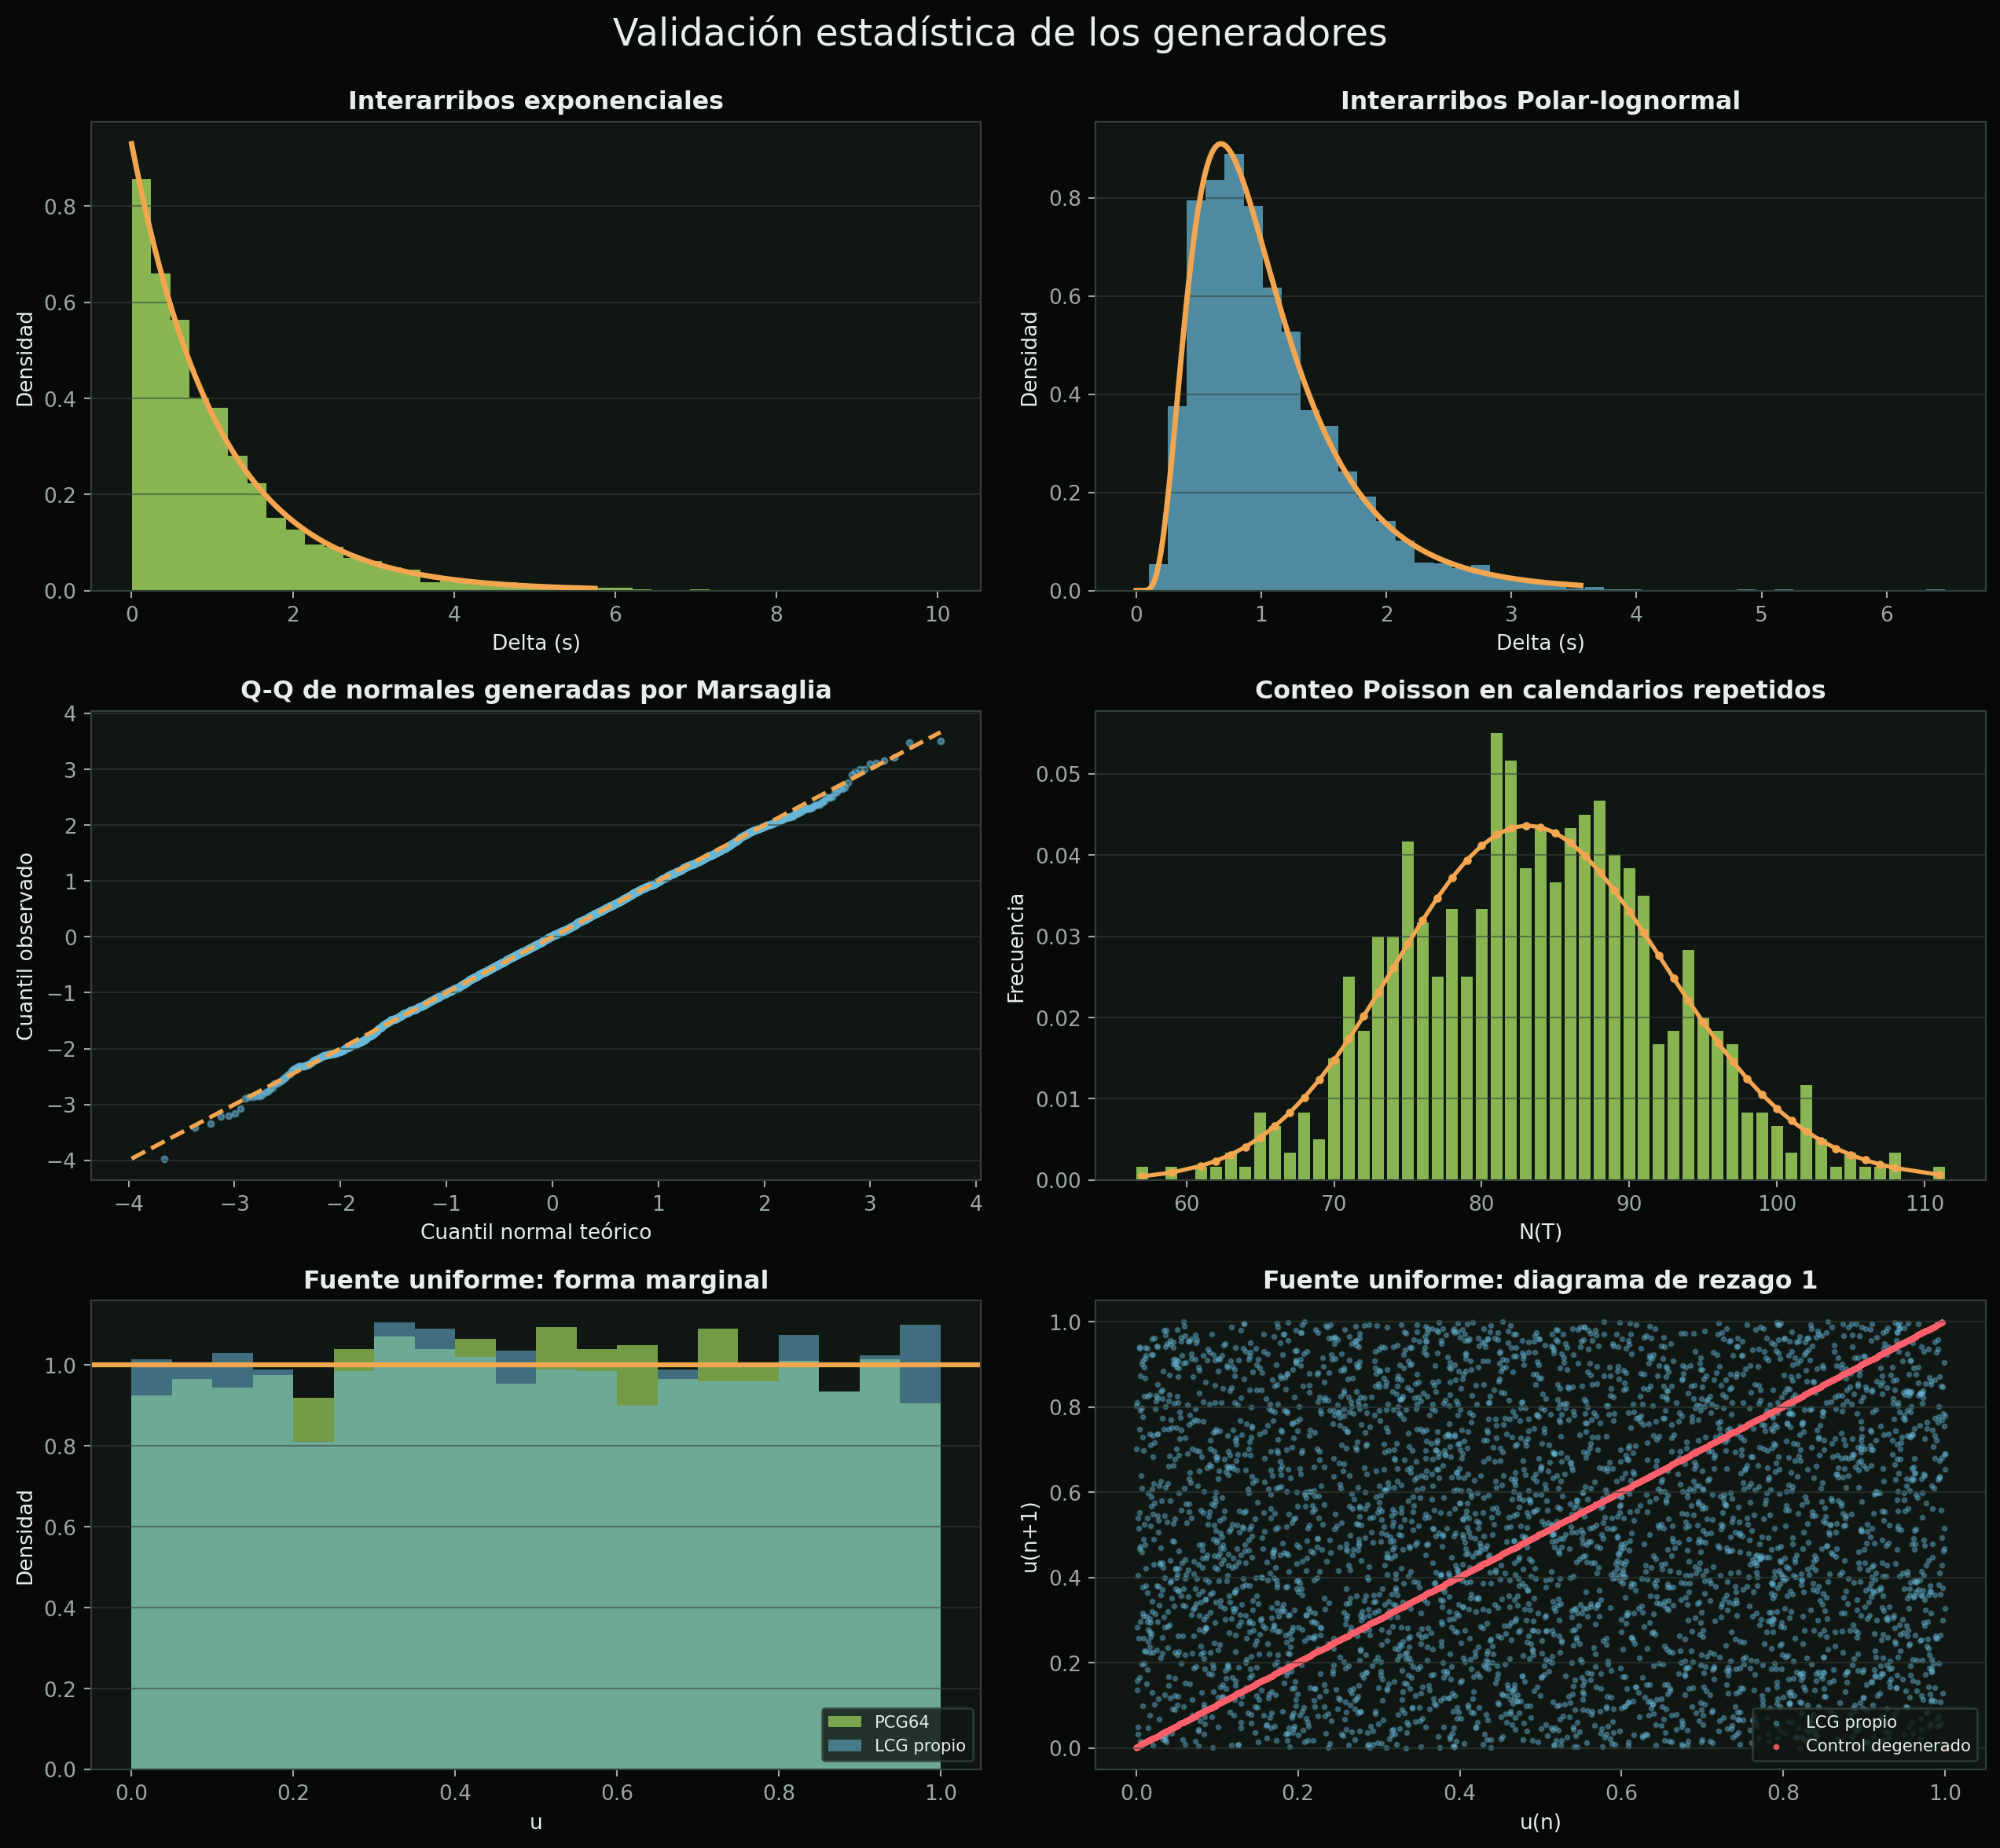
\includegraphics[width=\textwidth]{report-generator-validation.png}
  \caption{Histogramas, densidades, Q-Q normal, conteos Poisson y auditoría de
  la fuente uniforme. El diagrama de rezago uno, abajo a la derecha, contrapone
  el LCG propio con el control degenerado.}
  \label{fig:validation}
\end{figure}

\subsection{Control negativo}

Una batería que solo aprueba generadores correctos no demuestra nada mientras no
se compruebe que también reprueba a los defectuosos. Se somete a los mismos
contrastes un contador puro $x_{n+1}=(x_n+1)\bmod m$, que recorre su período
completo y es por construcción perfectamente uniforme, pero también
perfectamente predecible. El resultado separa dos propiedades que suelen
confundirse:

\begin{table}[H]
\centering
\caption{Control negativo: uniforme por construcción, jamás aleatorio.}
\begin{tabular}{lll}
\toprule
Contraste & Propiedad evaluada & Valor $p$ \\
\midrule
Ji-cuadrada de uniformidad & Forma marginal & \ControlUniformityP \\
KS contra $U(0,1)$ & Forma marginal & \ControlKSP \\
Rachas arriba/abajo & Orden secuencial & $\ControlRunsP$ \\
Ljung-Box rezagos 1--5 & Correlación conjunta & $\ControlLjungP$ \\
Serial de tercias & Estructura en el cubo & $\ControlSerialP$ \\
\bottomrule
\end{tabular}
\end{table}

El contador aprueba los dos contrastes de forma con valores $p$ cercanos a uno y
fracasa en los tres de dependencia. Esta asimetría es la justificación cuantitativa
de por qué la validación no se agota en un histograma: uniformidad y aleatoriedad
son propiedades distintas y exigen pruebas distintas.

\subsection{Costo de generación}

La mediana fue \PoissonMicros\ microsegundos por interarribo exponencial y
\PolarMicros\ microsegundos por valor Polar-lognormal. El benchmark depende
del equipo, pero evidencia el costo del rechazo y las transformaciones de Polar.

\subsection{Comparación directa Marsaglia Polar--Box--Muller}

Poisson--exponencial y Polar--lognormal no son dos algoritmos para una misma
variable: son dos modelos de llegada. Para aislar el método computacional se
generaron 20,000 observaciones $N(0,1)$ con Marsaglia Polar y con Box--Muller,
y se cronometraron nueve repeticiones vectorizadas. KS no rechazó ninguno
($p=\PolarNormalKSP$ y $p=\BoxMullerKSP$, respectivamente). Esos valores $p$
se usan como umbral de compatibilidad, no como ranking de calidad.

\begin{table}[H]
\centering
\caption{Dos métodos para la misma distribución normal estándar.}
\begin{tabular}{lrrrr}
\toprule
Método & KS $p$ & $\mu$s/valor & Rechazo & Puntaje / 5 \\
\midrule
Marsaglia Polar & \PolarNormalKSP & \PolarNormalMicros & \PolarRejectedPercent\,\% & \PolarMethodScore \\
Box--Muller & \BoxMullerKSP & \BoxMullerMicros & 0\,\% & \BoxMullerMethodScore \\
\bottomrule
\end{tabular}
\end{table}

La matriz pondera ajuste (0.30), costo (0.25), eficiencia y previsibilidad
(0.20), robustez numérica (0.15) y sencillez de auditoría (0.10). En el equipo
de referencia favorece a \NormalMethodWinner. El resultado de tiempo es
descriptivo y debe reproducirse en cada equipo. Polar sigue siendo pedagógicamente
pertinente porque materializa aceptación--rechazo y su tasa teórica $\pi/4$.

\begin{figure}[H]
  \centering
  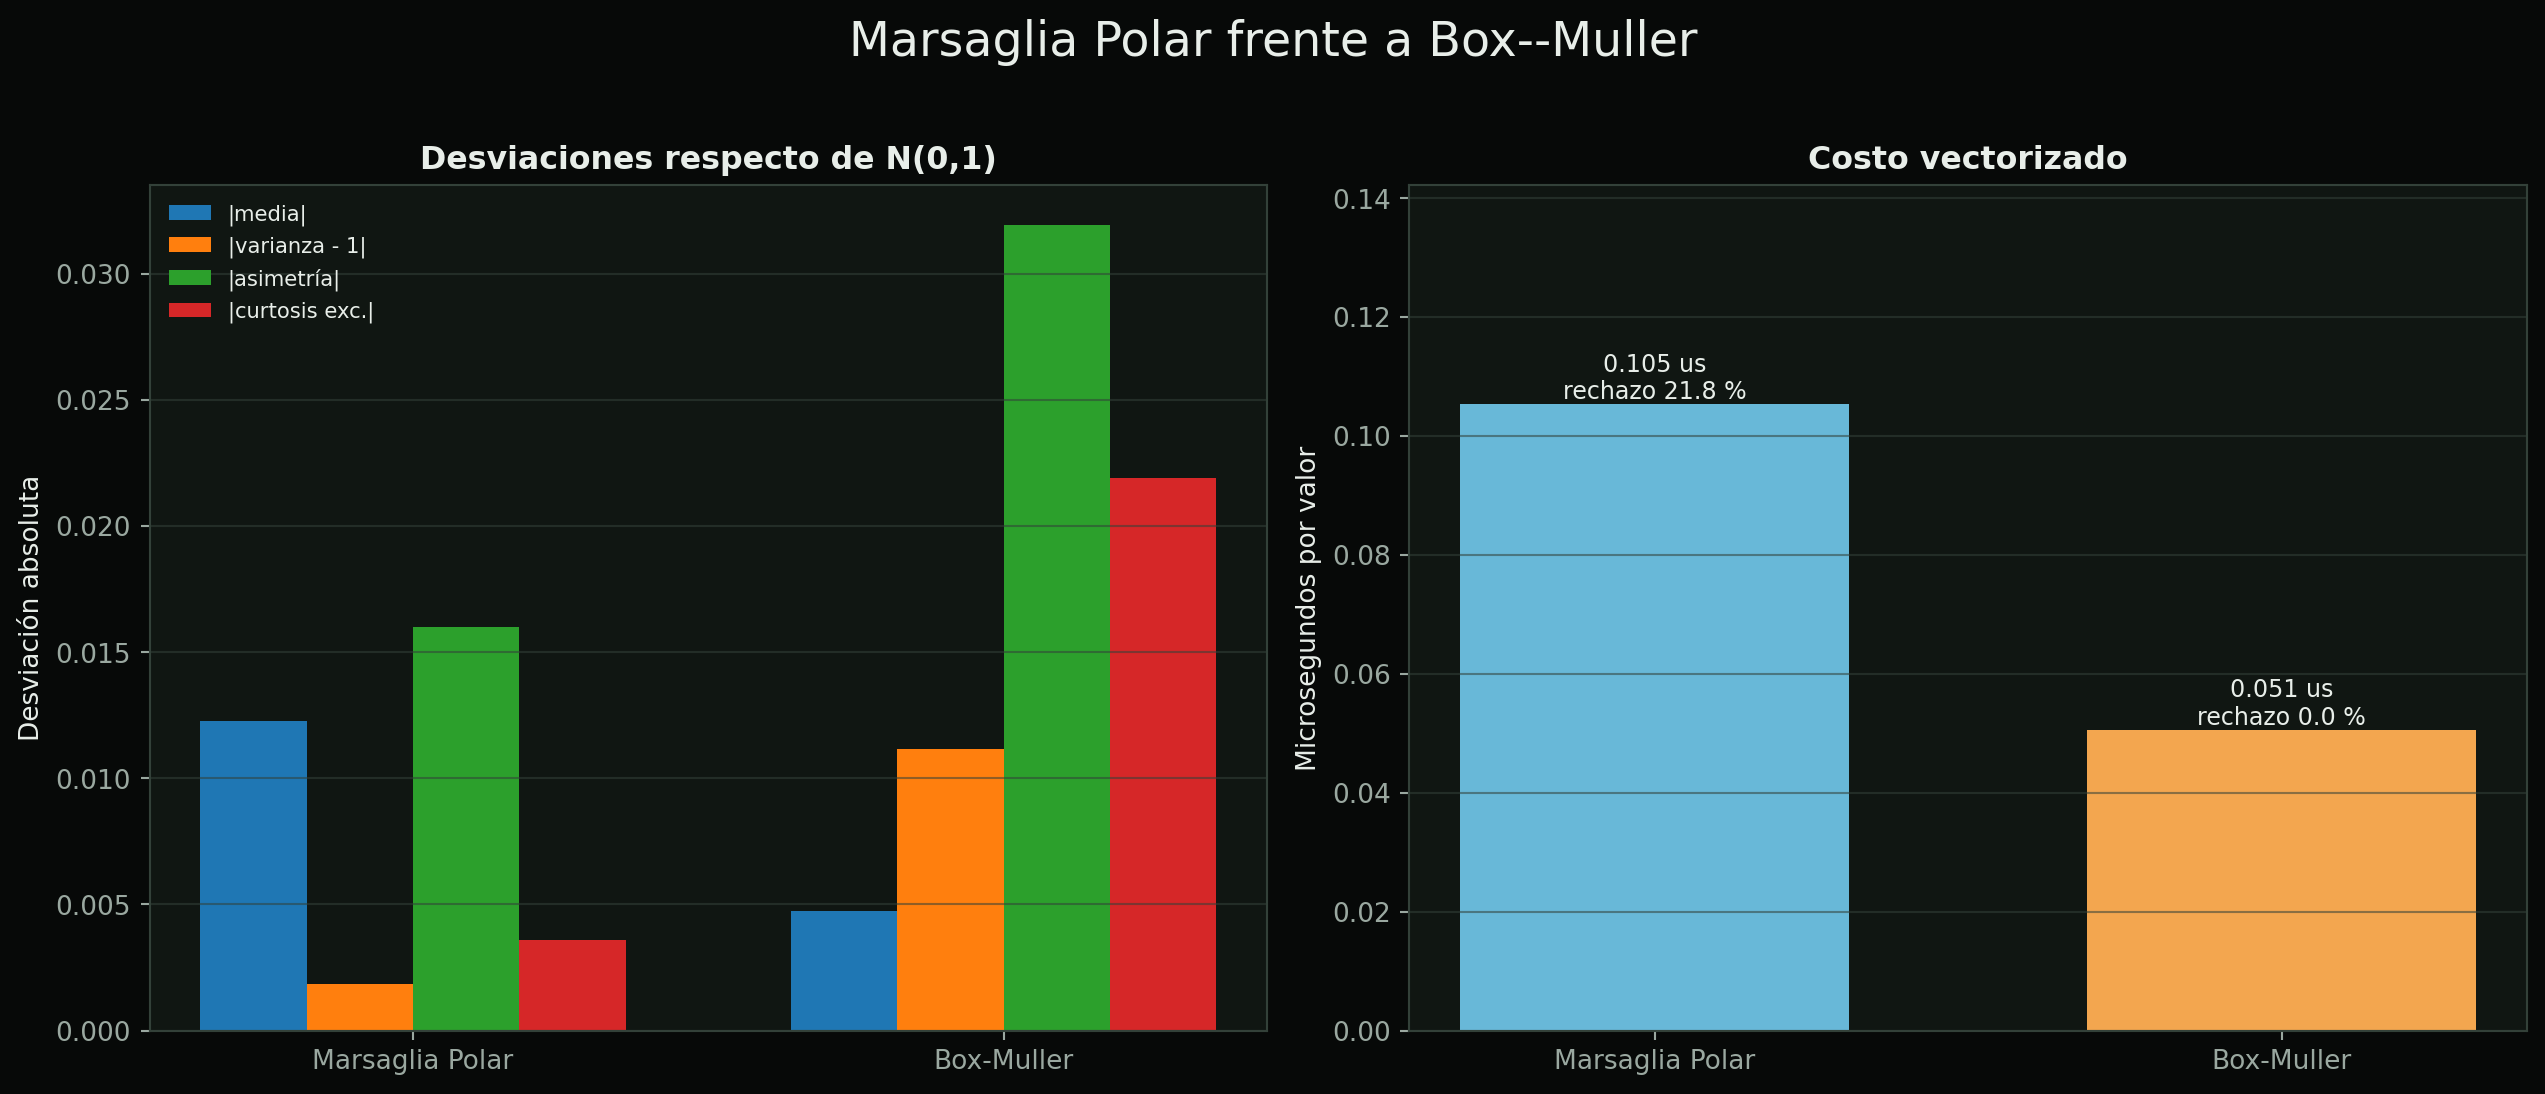
\includegraphics[width=\textwidth]{report-normal-method-comparison.png}
  \caption{Desviaciones de momentos y costo vectorizado para dos generadores de
  $N(0,1)$. No se ordenan métodos por el tamaño del valor $p$.}
  \label{fig:normal-methods}
\end{figure}

\subsection{Supervivencia y congestión}

\begin{table}[H]
\centering
\caption{Escenario base, 400 partidas por modelo.}
\label{tab:results}
\begin{tabular}{lrrrr}
\toprule
Modelo & $\widehat p$ (\%) & IC Wilson (\%) & Tiempo (s) & Pico \\
\midrule
Poisson & \PoissonSurvival & [\PoissonCILow, \PoissonCIHigh] &
\PoissonMeanTime & \PoissonPeak \\
Polar-lognormal & \PolarSurvival & [\PolarCILow, \PolarCIHigh] &
\PolarMeanTime & \PolarPeak \\
\bottomrule
\end{tabular}
\end{table}

\begin{table}[H]
\centering
\caption{Contingencia pareada.}
\begin{tabular}{lr}
\toprule
Resultado & Corridas \\
\midrule
Ambos sobreviven & \BothSurvive \\
Solo Poisson & \OnlyPoisson \\
Solo Polar & \OnlyPolar \\
Ambos fallan & \BothFail \\
\bottomrule
\end{tabular}
\end{table}

La diferencia fue \SurvivalDifference\ puntos porcentuales, con IC
[\SurvivalDiffLow, \SurvivalDiffHigh]. McNemar produjo $p=\McNemarP$:
existe evidencia de diferencia en este escenario. La concurrencia fue
\PeakDifference{} enemigos mayor bajo Poisson, con $p=\PeakP$.

\begin{figure}[H]
  \centering
  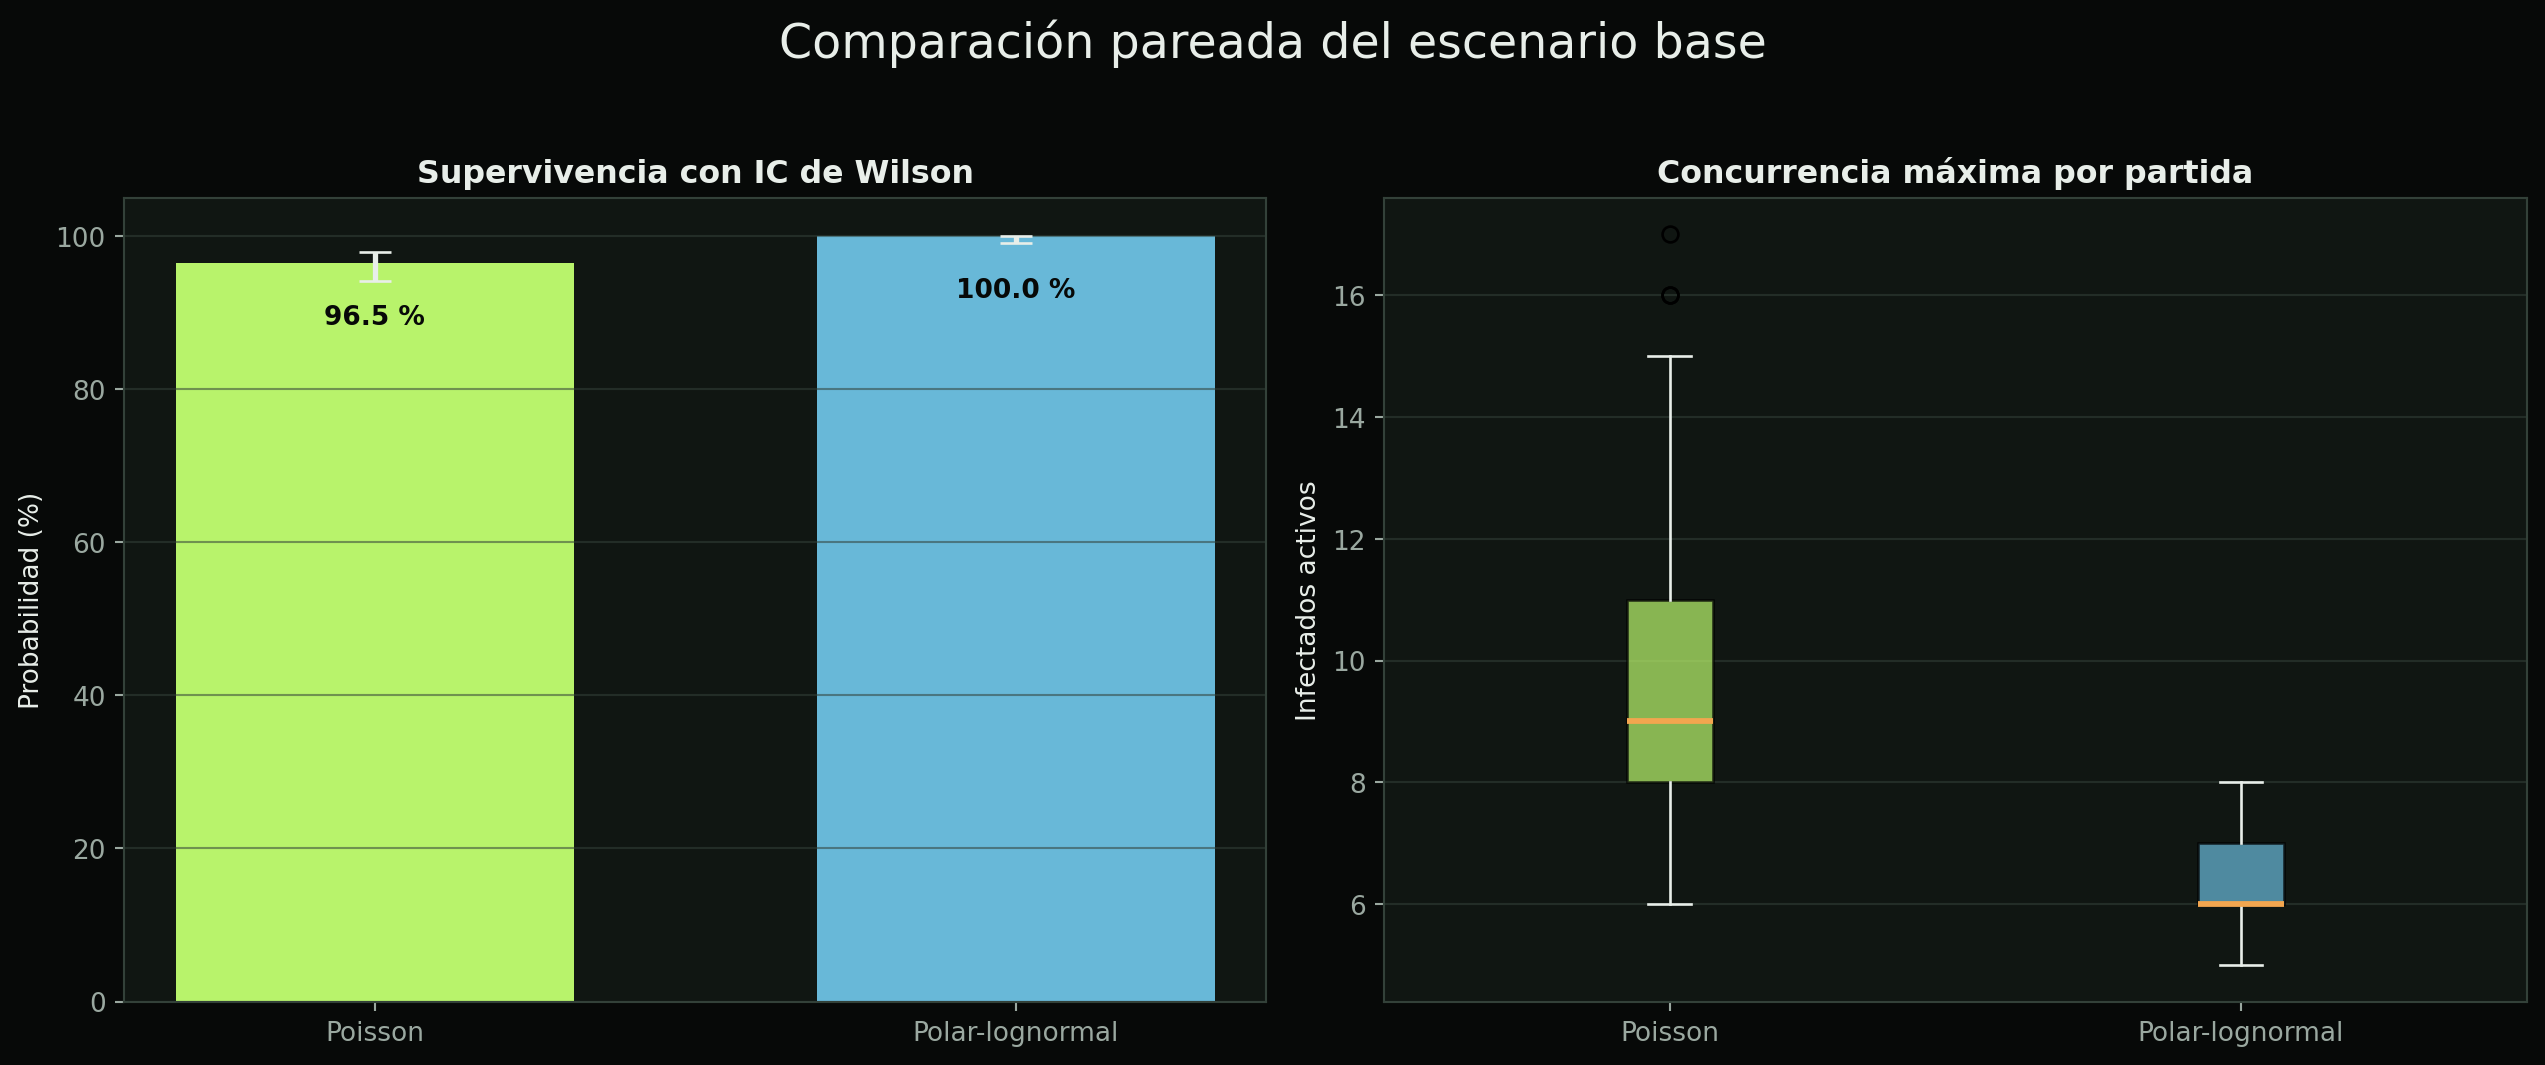
\includegraphics[width=\textwidth]{report-model-comparison.png}
  \caption{Supervivencia con Wilson y concurrencia máxima.}
  \label{fig:comparison}
\end{figure}

\subsection{Sensibilidad a la tasa}

\begin{figure}[H]
  \centering
  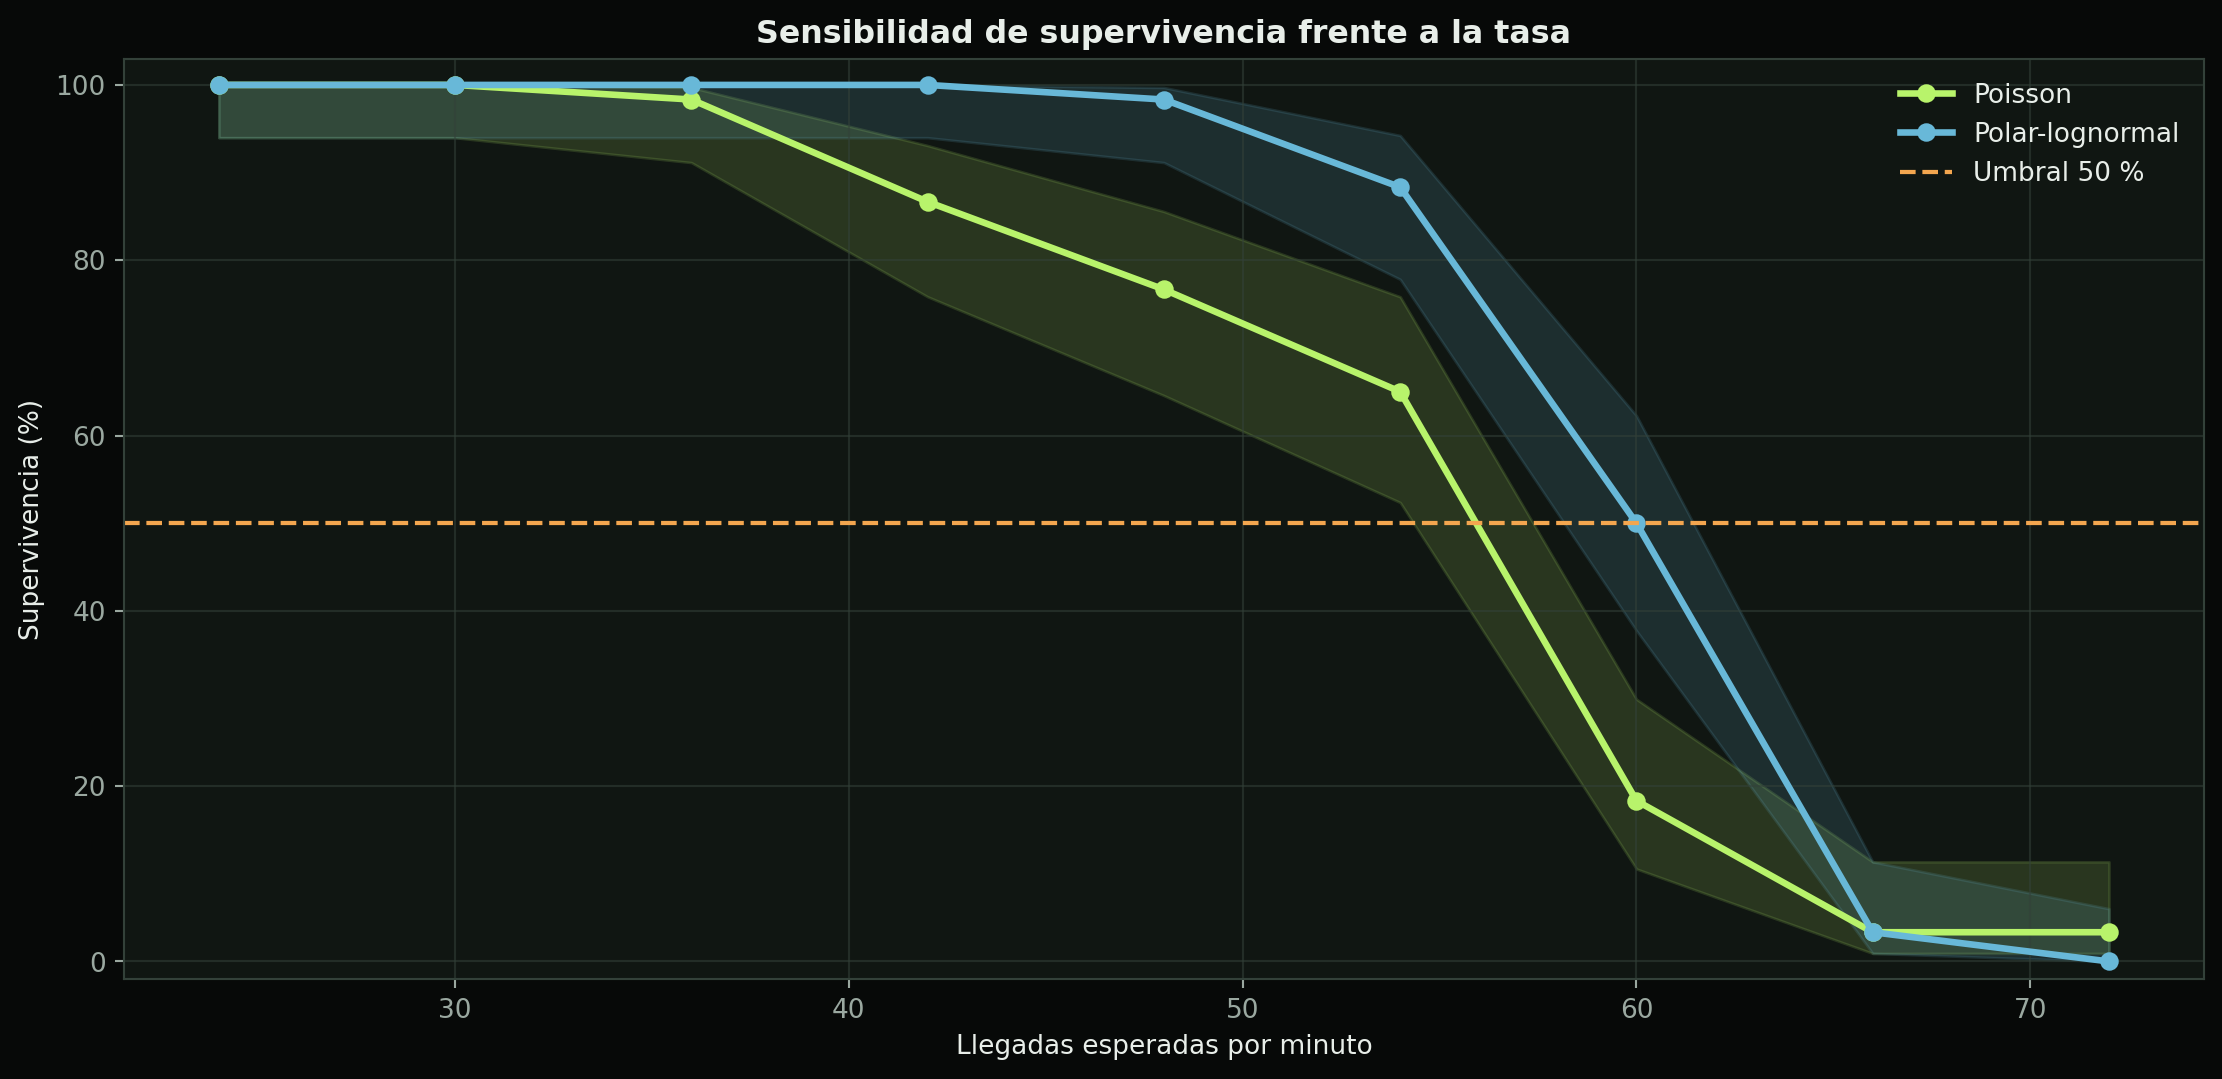
\includegraphics[width=0.96\textwidth]{report-survival-curves.png}
  \caption{Supervivencia para tasas de 24 a 72 llegadas/min.}
  \label{fig:curves}
\end{figure}

Una sola tasa no produce una conclusión universal. Al aumentar $\lambda$, la
presión supera la capacidad ofensiva y cae la supervivencia. Con CV 0.60,
Polar-lognormal retrasa rachas, pero esa ventaja pertenece al escenario.

\subsection{Trayectoria individual}

\begin{figure}[H]
  \centering
  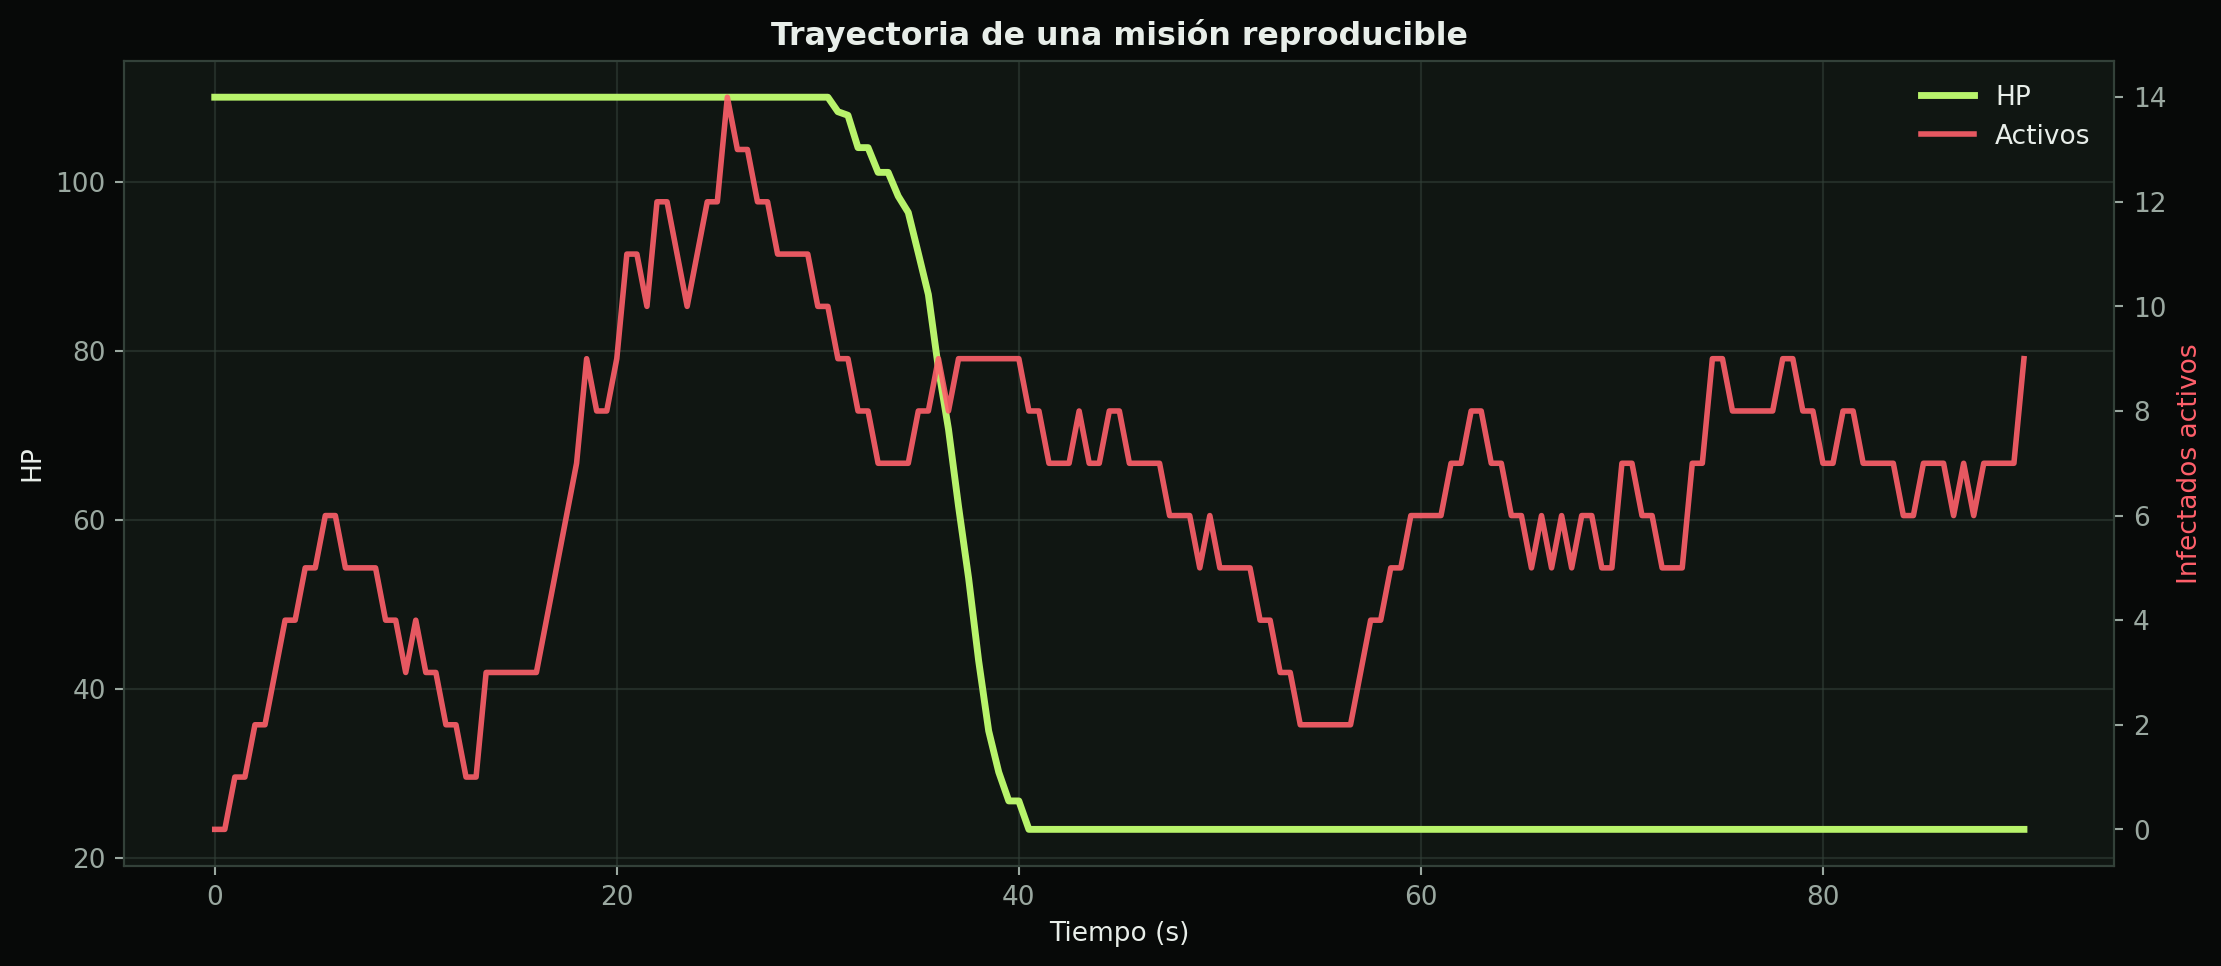
\includegraphics[width=0.94\textwidth]{report-timeline.png}
  \caption{HP y enemigos activos con semilla 22193.}
  \label{fig:timeline}
\end{figure}

La trayectoria explica causalidad entre rachas, concurrencia y daño; la
inferencia final se apoya en cientos de partidas.

\section{Análisis y elección}

\begin{table}[H]
\centering
\small
\caption{Matriz razonada de decisión.}
\begin{tabularx}{\textwidth}{>{\bfseries}p{2.8cm}XX}
\toprule
Criterio & Poisson-exponencial & Polar-lognormal \\
\midrule
Fundamento & Proceso de conteo exacto & Proceso de renovación \\
Ajuste & No rechazado & $Z$ normal y media calibrada \\
Interpretación & Un parámetro; relación exacta & Media y CV controlables \\
Costo & \PoissonMicros\ $\mu$s/valor & \PolarMicros\ $\mu$s/valor \\
Rachas & CV 1; mayor concurrencia & CV 0.60; mayor regularidad \\
Uso & Independencia y tasa constante & Datos con regularidad positiva \\
\bottomrule
\end{tabularx}
\end{table}

Poisson permanece como modelo principal por correspondencia con el conteo,
parsimonia, costo y supuestos. Polar-lognormal demuestra que igualar la media
no iguala congestión y resulta útil si datos observados exigen $CV\neq1$.
Sin telemetría real, la elección está condicionada por supuestos y no constituye
una verdad empírica sobre apocalipsis.

\section{Visualización y arquitectura}

Streamlit administra formulario, estado y caché; el motor numérico no depende
de Streamlit ni Plotly. \texttt{Mesh3d} construye una escena navegable con
personajes, ruinas, vehículos, barricadas y anillos tácticos.

\begin{figure}[H]
  \centering
  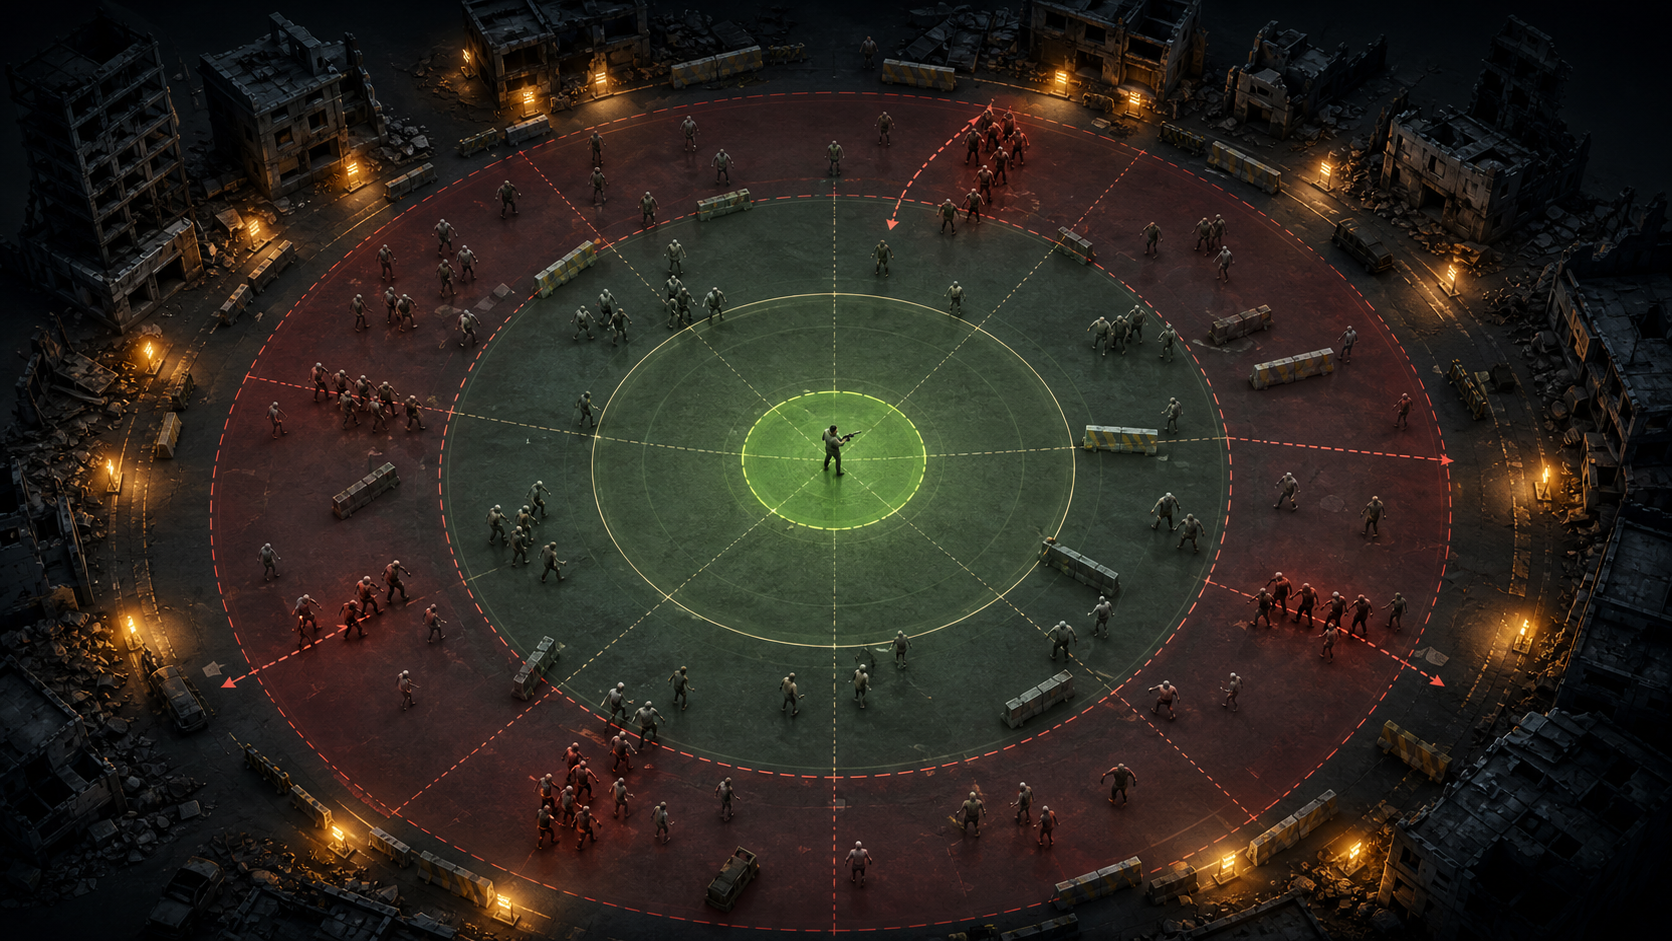
\includegraphics[width=0.82\textwidth]{outbreak-tactical-model.png}
  \caption{Aparición, alcance, contacto y presión en la arena.}
\end{figure}

Pygame no es requisito de la rúbrica y se orienta principalmente a superficies
2D. Un 3D de escritorio exigiría OpenGL u otro motor. Plotly conserva controles,
escena y evidencia en una aplicación web~\cite{plotly}. Panda3D es trabajo
futuro, no una deuda de esta entrega.

\section{Verificación}

La suite contiene 28 pruebas automatizadas. Sus familias son:

\begin{enumerate}
  \item reproducibilidad Poisson;
  \item media y varianza del conteo;
  \item media y positividad lognormal;
  \item los \TestCount{} contrastes de referencia bajo corrección de Holm;
  \item ausencia de estadísticos duplicados entre contrastes;
  \item separación del control negativo respecto de la tabla principal;
  \item reproducibilidad y rango del LCG propio;
  \item aceptación de la batería sobre la fuente de referencia;
  \item detección de dependencia en un generador uniforme pero predecible;
  \item corrección de Holm contra su cálculo manual y sus cotas;
  \item diseño de propuestas fijas para la prueba de aceptación;
  \item potencia de la ji-cuadrada del conteo ante una media desplazada;
  \item reproducibilidad de partida;
  \item separación de eventos programados y ocurridos;
  \item rechazo de geometría inválida;
  \item igualdad de semillas pareadas;
  \item estabilidad al reducir $dt$;
  \item ausencia de daño después de $T$;
  \item dirección y contingencia pareadas;
  \item límites del intervalo de Wilson;
  \item generación Polar vectorizada y su aceptación teórica;
  \item ajuste compartido de Polar y Box--Muller a $N(0,1)$;
  \item validez y ordenamiento de la matriz de decisión;
  \item escenario base no saturado y barrido de calibración.
\end{enumerate}

\texttt{streamlit.testing} verifica además carga, misión, validación,
comparación y Monte Carlo sin excepciones.

\section{Reproducibilidad}

Desde \texttt{zombie\_poisson\_streamlit}:

\begin{verbatim}
python -m pip install -r requirements/requirements.txt
python -m unittest discover -s tests -v
python report/generate_report_assets.py
python -m streamlit run App/app.py
\end{verbatim}

Las versiones están fijadas y los CSV permiten auditar números sin abrir la UI.
Para recompilar:

\begin{verbatim}
cd report
pdflatex informe.tex
pdflatex informe.tex
\end{verbatim}

\section{Supuestos y limitaciones}

\begin{enumerate}
  \item La tasa es constante dentro de cada partida.
  \item Independencia es un supuesto de diseño, no una conclusión de datos.
  \item El protagonista es estacionario y enfoca un objetivo.
  \item No hay colisiones ni evitación de obstáculos.
  \item El combate usa paso finito; la convergencia cubre un caso sencillo.
  \item La variación uniforme de atributos no tiene calibración empírica.
  \item KS depende del tamaño; se complementa con momentos y Q-Q.
  \item El LCG propio se audita, pero no sustituye a PCG64 dentro del motor:
        su papel es servir de término de comparación con evidencia.
  \item El control negativo demuestra potencia frente a dependencia secuencial;
        no cubre todas las formas posibles de defecto.
  \item Valores $p$ no miden importancia práctica; se reportan efectos e IC.
  \item El benchmark depende del equipo.
  \item Las curvas Monte Carlo usan una cuadrícula finita.
  \item Las ruinas son visuales y no alteran trayectorias.
\end{enumerate}

\section{Conclusiones}

\begin{enumerate}
  \item Los \TestCount{} contrastes fueron coherentes con los generadores
        declarados, incluida la fuente uniforme que ambos métodos comparten, y
        no se duplicó un mismo estadístico como si fuera evidencia adicional.
  \item El control negativo confirma que la batería distingue uniformidad de
        aleatoriedad: un contador aprueba los contrastes de forma y fracasa en
        los de dependencia.
  \item Igual media no produjo igual concurrencia: Poisson generó un pico medio
        aproximadamente tres enemigos mayor.
  \item El diseño pareado encontró diferencia de supervivencia en el escenario
        base sin convertirla en superioridad universal.
  \item Poisson es principal por coherencia, parsimonia, costo e interpretación.
  \item Polar-lognormal es valioso cuando interesa controlar el CV.
  \item En el benchmark reproducible, Box--Muller obtuvo el mayor puntaje al
        generar la misma normal; Polar conserva valor didáctico y experimental.
  \item La corrección temporal impide daño después del horizonte.
  \item App, CSV, figuras, informe y presentación usan evidencia reproducible.
\end{enumerate}

\section{Trabajo futuro}

Se propone calibrar $\lambda$ y atributos con telemetría real, evaluar Poisson
no homogéneo $\lambda(t)$, estudiar conjuntamente CV y combate, permitir
movimiento, hacer funcionales los obstáculos y crear una versión Panda3D. Estas
extensiones no son necesarias para cumplir la rúbrica actual.

\begin{thebibliography}{9}
\bibitem{ross}
S. M. Ross, \textbf{Simulation}, Academic Press.

\bibitem{devroye}
L. Devroye, \textbf{Non-Uniform Random Variate Generation}, Springer, 1986.

\bibitem{marsaglia}
G. Marsaglia y T. A. Bray, \textbf{A convenient method for generating normal
variables}, SIAM Review, 1964.

\bibitem{wilson}
E. B. Wilson, \textbf{Probable inference, the law of succession, and
statistical inference}, JASA, 1927.

\bibitem{efron}
B. Efron y R. Tibshirani, \textbf{An Introduction to the Bootstrap},
Chapman \& Hall/CRC, 1993.

\bibitem{plotly}
Plotly, \textbf{3D Mesh Plots in Python}.\\
\url{https://plotly.com/python/3d-mesh/}
\end{thebibliography}

\end{document}
